%%%%%%%%%%%% MAIN PACKAGES %%%%%%%%%%%%
\documentclass{template}
\usepackage[T1]{fontenc}
\usepackage{lmodern}
\usepackage{graphicx,parskip,appendix,float}
\usepackage[ruled,vlined]{algorithm2e}
\usepackage{url,amsmath,amssymb,booktabs,tabularx,longtable,array}
\usepackage{listings,caption,csquotes,microtype}
\usepackage{tikz}
\usetikzlibrary{arrows.meta,positioning,shapes.geometric}
\usepackage{placeins}
\ifdefined\LocalBuild
  \usepackage[style=authoryear,giveninits=true,uniquename=init,backend=bibtex,maxcitenames=2,maxbibnames=10]{biblatex}
\else
  \usepackage[style=authoryear,giveninits=true,uniquename=init,backend=biber,maxcitenames=2,maxbibnames=10]{biblatex}
\fi
\addbibresource{thesis.bib}
\AtBeginBibliography{\raggedright}
\usepackage[pagebackref=false,pdffitwindow=true]{hyperref}
% Edit report details here; they are reused on the title and certificate pages.
\newcommand{\ReportTitle}{Simulation-Based Evaluation of UAV Navigation Using PPO and Adaptive Control Barrier Functions}
\newcommand{\AuthorName}{Tridibesh Sarkar}
\newcommand{\StudentNumber}{23AE30023}
\newcommand{\SupervisorName}{Prof. Priyam Chakraborty}
\newcommand{\DepartmentName}{Aerospace Engineering}
\newcommand{\InstituteName}{Indian Institute of Technology Kharagpur}
\title{\ReportTitle}
\author{\AuthorName}
\studentnumber{\StudentNumber}
\degreetitle{Dual Degree}
\rpttype{B.Tech. Project}
\principaladviser{\SupervisorName}
\department{\DepartmentName}
\institute{\InstituteName}
\date{November 2026}

\hypersetup{pdftitle={\ReportTitle},pdfauthor={\AuthorName},
 pdfsubject={UAV navigation, reinforcement learning and safety filtering},
 colorlinks=true,linkcolor=blue,citecolor=blue,urlcolor=blue}
\graphicspath{{figures/}}
\DeclareGraphicsExtensions{.pdf,.png,.jpg}
\captionsetup{font=small,labelfont=bf}
\setlength{\emergencystretch}{2em}
\setlength{\tabcolsep}{5pt}
\renewcommand{\arraystretch}{1.15}
\newcolumntype{Y}{>{\raggedright\arraybackslash}X}
\newcommand{\R}{\mathbb{R}}
\newcommand{\norm}[1]{\left\lVert#1\right\rVert}
\newcommand{\selectedsteps}{630,000}
\newcommand{\finalsteps}{670,000}
\lstset{language=Python,basicstyle=\ttfamily\small,breaklines=true,
 frame=single,numbers=left,numberstyle=\tiny,showstringspaces=false,
 captionpos=b,columns=fullflexible}
\begin{document}
\hypersetup{pageanchor=false}
\maketitle
\pagenumbering{roman}
\hypersetup{pageanchor=true}
\chapter*{Certificate}
\addcontentsline{toc}{chapter}{Certificate}
\markboth{Certificate}{Certificate}
This is to certify that the project report entitled
\textbf{\textquotedblleft\ReportTitle\textquotedblright}, submitted by
\textbf{\AuthorName} (\StudentNumber) to the Department of \DepartmentName,
\InstituteName, is a record of bona fide work carried out under my supervision
and guidance.

\vspace{3cm}
\noindent\begin{tabular}{@{}l}
\rule{6cm}{0.4pt}\\
\SupervisorName\\
Department of \DepartmentName\\
\InstituteName
\end{tabular}
\hfill Date: \rule{3cm}{0.4pt}

\chapter*{Abstract}\addcontentsline{toc}{chapter}{Abstract}
Autonomous unmanned aerial vehicles must achieve navigation objectives while maintaining adequate separation from moving obstacles. A reinforcement-learning policy can learn useful motion commands, but successful goal reaching alone does not establish obstacle safety. This project implements and evaluates a paper-inspired hierarchical controller that combines proximal policy optimization (PPO), an interacting multiple model (IMM) obstacle predictor, and an adaptive control barrier function (ACBF) filter. The evaluation uses a Crazyflie CF2X model in PyBullet and compares pure PPO, the same PPO with IMM and ACBF, and a classical PID-based reference controller with the same filter.

The implementation uses a 19-dimensional observation, bounded net-acceleration commands, an inner attitude loop, and a staged goal-distance curriculum. A fresh eight-environment training run with a two-million-transition budget stopped at 670,000 transitions after satisfying its repeated-validation condition. The automatically selected and validated checkpoint, saved at 630,000 transitions, is used for the main scenario results. Both this checkpoint and the final checkpoint reached 59 of 60 additional evaluation goals. The remaining target produced a small but persistent position error outside the predefined 0.10~m success radius.

All three controllers reached the shared goal in the linear, accelerating and figure-eight obstacle scenarios. For the selected checkpoint in the figure-eight case, pure PPO entered the 0.50~m safety buffer, attaining a minimum centre distance of 0.464~m. PPO with ACBF maintained 0.770~m and reached the goal in 13.60~s, compared with 13.70~s for pure PPO. The PID-based baseline was faster, reaching the same goal in 7.80~s. These experiments demonstrate effective integration and an observed safety-buffer benefit, while exposing remaining limitations in goal generalization, numerical timing and prediction robustness. The results concern one training seed and a finite set of simulated trials; they do not constitute a general safety guarantee or hardware validation.

\noindent\textbf{Keywords:} UAV navigation; proximal policy optimization; interacting multiple model; adaptive control barrier function; safety filtering; PyBullet.

\tableofcontents
\listoffigures
\listoftables
\listofalgorithms
\chapter*{Abbreviations and Notation}\addcontentsline{toc}{chapter}{Abbreviations and Notation}
\begin{tabularx}{\textwidth}{lY}
\toprule Symbol / abbreviation & Meaning\\\midrule
UAV & Unmanned aerial vehicle\\
RL / PPO & Reinforcement learning / proximal policy optimization\\
IMM & Interacting multiple model estimator\\
CV / CA / CT & Constant-velocity / constant-acceleration / coordinated-turn model\\
CBF / ACBF & Control barrier function / adaptive control barrier function\\
PID & Proportional--integral--derivative controller\\
$p,v$ & UAV position and velocity in the inertial frame\\
$p_g,p_o$ & Goal position and obstacle centre position\\
$u_{\rm ref},u$ & Nominal and filtered net-acceleration commands\\
$\Delta t,N$ & Control interval and prediction horizon\\
$d,d_c,d_s$ & Centre separation, collision threshold and safety boundary\\
$e$ & Euclidean position error to the goal\\
$h_i,\psi_i$ & Predicted barrier value and first-order discrete barrier difference\\
$\gamma$ & Adaptive barrier coefficient; distinct from PPO's discount factor\\
$\beta$ & PPO reward-discount factor, denoted \texttt{ppo\_gamma} in code\\
$\xi,\delta$ & Nonnegative higher-order and coefficient-update relaxation variables\\
\bottomrule
\end{tabularx}

\clearpage\pagenumbering{arabic}
\chapter{Introduction}\label{ch:introduction}
\section{Motivation}
Drone navigation in a dynamic environment involves two related requirements: moving toward the destination and preserving separation from obstacles. A controller can satisfy one requirement while failing the other. For example, remaining stationary may avoid an obstacle but fail the mission, while a fast direct trajectory may reach the goal after passing too close to another object. An evaluation should therefore measure arrival, final tracking error, obstacle separation and computational cost together.

Learning-based navigation is attractive because the mapping from state to control can be improved through interaction with a simulator. However, the resulting policy is not automatically a reliable obstacle-avoidance controller. In this project, PPO learns goal-directed motion, while an explicit lower layer uses predicted obstacle motion to modify commands. The design follows the hierarchical idea of \textcite{gao2026}, with implementation adaptations documented throughout this report.

\section{Problem statement}
The simulated system consists of one quadrotor and one moving spherical obstacle. The drone starts from a prescribed position and must enter a goal neighborhood within a finite episode. The nominal policy outputs bounded three-dimensional acceleration commands. The safety layer receives the drone state and an estimate of the obstacle trajectory, and attempts to preserve a prescribed separation while remaining close to the nominal command.

The central research question is: \emph{Can a prediction-based adaptive safety filter improve measured obstacle separation while retaining the goal-reaching behavior of a learned navigation policy?} A second question concerns the cost of that filter in mission time, path length and computation. A third concerns the relationship between successful benchmark trajectories and generalization to other destinations.

\section{Objectives and scope}
The project has four objectives. First, it establishes a consistent interface between PPO, the drone dynamics and the safety filter. Second, it implements obstacle-state estimation and finite-horizon filtering. Third, it compares pure RL, RL with ACBF, and a classical controller with the same ACBF layer. Finally, it evaluates learning progress and investigates failures rather than treating every saved model as converged.

The scope is a simulation study with one drone, one obstacle, prescribed obstacle trajectories and exact simulated obstacle-position measurements. The estimator still uses process and measurement covariance assumptions, but a realistic noisy sensing pipeline is not evaluated. Multi-drone coordination, multiple simultaneous obstacles, wind disturbances and physical flight tests are outside the demonstrated scope.

\section{Project contribution}
The contribution is an implementation and empirical evaluation of a paper-inspired control architecture. It includes a versioned policy interface, consistent plant forecasts, a curriculum-based training procedure, recorded success and safety diagnostics, and checkpoint comparisons that expose residual position bias. It is not a claim of a new PPO algorithm or a new formal barrier-function theorem.

The evidence is deliberately separated into three levels. The training logs show whether the configured validation objective is reached. Additional goal tests examine behavior beyond the callback's fixed goal set. Moving-obstacle tests examine the interaction between navigation and filtering. A strong result at one level is not treated as proof at the other levels.

\section{Organization of the report}
Chapter~\ref{ch:background} introduces the relevant learning and control concepts. Chapter~\ref{ch:design} formulates the implemented navigation and filtering problem. Chapter~\ref{ch:implementation} describes the software, training and evaluation procedures. Chapter~\ref{ch:evaluation} reports the measured results and limitations. Chapter~\ref{ch:conclusion} presents conclusions and future work. Appendix~\ref{app:repro} records provenance, reproduction commands and the figure inventory.

\chapter{Background and Related Work}\label{ch:background}
\section{Reinforcement learning and PPO}
A policy maps observations to actions, and training adjusts the policy to improve expected return. Let $o_t$ denote an observation, $a_t$ an action and $r_t$ a reward. With discount factor $\beta$, the return is $G_t=\sum_{j=0}^{\infty}\beta^j r_{t+j}$. A higher return is useful only insofar as the reward and evaluation criteria reflect the intended task.

PPO limits policy changes using a clipped probability-ratio objective \parencite{schulman2017}. Writing $\rho_t(\theta)=\pi_\theta(a_t\mid o_t)/\pi_{\theta_{\rm old}}(a_t\mid o_t)$ and $\hat A_t$ for an estimated advantage, the policy objective is
\begin{equation}
L^{\rm clip}(\theta)=\mathbb{E}_t\!\left[\min\!\left(\rho_t(\theta)\hat A_t,
\operatorname{clip}(\rho_t(\theta),1-\epsilon,1+\epsilon)\hat A_t\right)\right].
\end{equation}
The present implementation uses Stable-Baselines3 rather than a new implementation of PPO \parencite{raffin2021}. Training samples stochastic actions; the reported policy evaluations use deterministic actions. Consequently, success over a training episode window and success of the final deterministic policy are related but different measurements.

\section{Safety filtering}
A safety filter modifies a nominal control command using constraints derived from the system state. The nominal controller retains responsibility for task progress. Barrier-function methods provide a mathematical language for describing a safe set and restricting control inputs to maintain it under appropriate assumptions \parencite{ames2017}. Those assumptions include the dynamics, available control authority and feasibility of the constraints.

In a numerical implementation, finite sampling, state-estimation error and approximate optimization must also be considered. Therefore a barrier-inspired controller operating successfully in a few simulations is not itself a proof of forward invariance. This report uses measured geometric separation to assess the local implementation and explicitly records cases where prediction or feasibility limits have appeared.

\section{Obstacle prediction with multiple models}
One motion model may not describe every phase of an obstacle trajectory. A constant-velocity model is suitable for straight motion, a constant-acceleration model represents changes in speed, and a coordinated-turn model represents changing heading. The local IMM predictor combines these alternatives by mixing their state estimates, performing model-specific updates, updating model probabilities and fusing the resulting predictions. This is the predictor structure adopted from the source architecture \parencite{gao2026}.

The combination is useful for a finite prediction horizon, but its output remains an estimate. A small error matters when a predicted trajectory passes close to the safety boundary. The study therefore distinguishes predicted separation from the separation measured after the simulator executes the command.

\section{Simulation platform and classical baseline}
The \texttt{gym-pybullet-drones} environment provides quadrotor simulation and control components suitable for learning experiments \parencite{panerati2021}. This project builds a custom navigation environment around its Crazyflie model. The actual control command is converted to rotor inputs using an inner attitude controller; the vehicle is not advanced solely by an ideal point-mass equation.

A position-error controller provides a classical comparison. It is labelled PID+ACBF to retain the repository terminology, although the evaluated position gains set the integral term to zero. Thus its outer navigation law is effectively proportional--derivative control. All three methods share the same simulated plant and stopping criterion.

\section{Relationship to the source paper}
\textcite{gao2026} motivates the combination of learned reference commands, IMM prediction and adaptive barrier filtering. The present work evaluates that structural idea, not an exact reproduction of every reported paper experiment. The local policy has expanded observations, net-acceleration semantics, an explicit curriculum and additional reward terms. A single PPO checkpoint is used in both RL variants across all three obstacle cases. These choices make the effect of adding the filter observable for a fixed policy, but do not reproduce comparisons involving separately trained case-specific policies.

No numerical superiority claim is transferred from the source paper to this implementation. In particular, the local PID baseline remains faster, and the observed safety benefit is reported using explicit centre-distance thresholds. Claims about universal safety, adaptation benefits relative to a fixed CBF, or the independent contribution of IMM require further analysis and experiments.

\chapter{System Design and Mathematical Formulation}\label{ch:design}
\section{Hierarchical architecture}
Figure~\ref{fig:architecture} shows the implemented information flow. PPO proposes a nominal command from the drone observation. The IMM processes obstacle positions independently of PPO. The ACBF layer combines the predicted obstacle trajectory with candidate drone trajectories to select a bounded command. The inner controller converts that command into rotor inputs. In the pure-RL comparison, the nominal command bypasses the IMM/ACBF layer; the observation and PPO weights are unchanged.

\begin{figure}[htbp]\centering
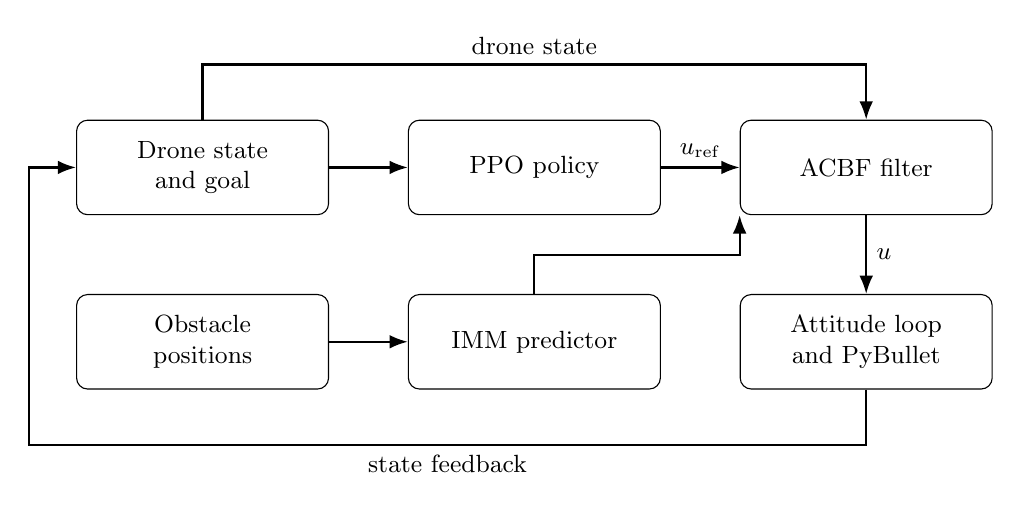
\begin{tikzpicture}[font=\small,box/.style={draw,rounded corners,align=center,minimum width=32mm,minimum height=12mm},arr/.style={-{Latex},thick},node distance=10mm and 10mm]
\node[box] (state) {Drone state\\and goal};
\node[box,right=of state] (ppo) {PPO policy};
\node[box,right=of ppo] (filter) {ACBF filter};
\node[box,below=of state] (obs) {Obstacle\\positions};
\node[box,right=of obs] (imm) {IMM predictor};
\node[box,below=of filter] (plant) {Attitude loop\\and PyBullet};
\draw[arr] (state)--(ppo);\draw[arr] (ppo)--node[above]{$u_{\rm ref}$}(filter);
\draw[arr] (obs)--(imm);\draw[arr] (imm.north)--++(0,5mm)-|(filter.south west);
\draw[arr] (state.north)--++(0,7mm)-|node[pos=.25,above]{drone state}(filter.north);
\draw[arr] (filter)--node[right]{$u$}(plant);
\draw[arr] (plant.south)--++(0,-7mm)-|node[pos=.25,below]{state feedback}([xshift=-6mm]state.west)--(state.west);
\end{tikzpicture}
\caption{Implemented hierarchy. The safety layer is used during evaluation; PPO training uses goal-navigation episodes with a distant obstacle.}\label{fig:architecture}
\end{figure}

\section{State, observation and action}
Let $p,v\in\R^3$ denote inertial position and velocity, and let $p_g$ denote the target. The position error is $p_g-p$. A conceptual translational model is
\begin{equation}
\dot p=v,\qquad \dot v=-g e_3+\frac{T}{m}R e_3,
\end{equation}
where $R$ maps body-frame vectors to the inertial frame and $T$ is total rotor thrust. The actual simulator includes rotational dynamics and the inner controller; this equation is not a replacement for the simulated plant.

The normalized policy action $a\in[-1,1]^3$ is mapped to net acceleration $u=k_{ma}a$, subject to the effective command bounds. Here $k_{ma}=1$, giving an effective per-axis range of $[-1,1]$~m/s$^2$. Although the configuration also contains nominal bounds of $[-3,3]$, the implementation intersects them with the normalized action range. The desired force is $m(u+g e_3)$, so gravity is added once. A zero net-acceleration command corresponds to a level hover in the ideal stationary case.

The 19-dimensional observation is
\begin{equation}
o=\left[\frac{v}{2},\ \frac{p_g-p}{5},\ \frac{\eta}{\pi},\
\frac{\omega}{10},\ \frac{\eta_{\rm prev}}{\pi},\ \frac{p}{10},\ f_h\right],
\end{equation}
where $\eta$ is roll--pitch--yaw, $\omega$ is angular velocity, $\eta_{\rm prev}$ is stored inner-controller attitude history and $f_h$ is the fraction of the required goal-hold interval completed. The fixed scales are part of the checkpoint interface. Obstacle position is not included. Absolute position provides information relevant to flight bounds, but also allows location-dependent policies; its effect is revisited in the evaluation.

\section{Navigation reward and stopping criterion}
Let $e_t=\norm{p_g-p_t}$, $I_g$ indicate successful arrival and $I_b$ indicate a flight-boundary failure. The implemented reward is
\begin{align}
r_t={}&100I_g+5(e_{t-1}-e_t)-10I_b-0.1\Delta t\nonumber\\
&-0.5e_t\Delta t-0.1\norm{v_t}^2\Delta t.
\label{eq:reward}
\end{align}
The first four terms follow the terminal/progress/boundary/time structure used in the source approach. The distance and speed costs and the chosen scaling are local adaptations. The speed cost is intended to discourage excessive motion, while the terminal reward distinguishes arrival from merely approaching the destination. These design intentions are assessed through actual success measurements rather than assumed to guarantee convergence.

Arrival requires $e_t<0.10$~m and $\norm{v_t}\leq0.20$~m/s for five consecutive 20~Hz control samples. The episode limit is 500 samples, or 25~s. Leaving the configured flight bounds or dropping below 0.05~m altitude is a terminal failure. A time limit is a truncation. Geometric obstacle collision is recorded by the evaluator; it is not conflated with the goal or boundary stopping rule. An episode can therefore reach a goal while still having a safety violation in its recorded trajectory.

\section{IMM prediction}
The implementation maintains native CV, CA and CT states of dimensions 6, 9 and 7, respectively. Mixing is performed through a common nine-dimensional position--velocity--acceleration representation. If $\mu_i$ denotes the prior probability of model $i$ and $\Pi_{ij}$ the transition probability, then
\begin{equation}
\bar c_j=\sum_i\Pi_{ij}\mu_i,\qquad
\mu_{i\mid j}=\frac{\Pi_{ij}\mu_i}{\bar c_j}.
\end{equation}
Mixed means and covariances initialize the model-specific updates. Measurement likelihoods update the mode probabilities. Each model is then propagated independently over the horizon, and predicted positions are fused using the current probabilities:
\begin{equation}
\hat p_{o,k+i\mid k}=\sum_j\mu_j(k)\hat p^{(j)}_{o,k+i\mid k}.
\end{equation}
The transition matrix has diagonal entries 0.6 and off-diagonal entries 0.2. Process and position-measurement covariance scales are both 0.05. The prediction horizon is $N=5$, corresponding to 0.25~s. This weighted forecast is not an uncertainty envelope.

\section{Geometry and adaptive barrier conditions}
The geometric centre separation is $d=\norm{p-p_o}$. With configured drone and obstacle radii of 0.2~m and a 0.1~m cushion,
\begin{equation}
d_c=0.4\ \mathrm{m},\qquad d_s=0.5\ \mathrm{m}.
\end{equation}
A collision proxy is recorded when $d\leq d_c$; a buffer violation is recorded when $d<d_s$. Surface clearance is $d-d_c$. These definitions are kept distinct in every results table.

For predicted positions at horizon index $i$, define
\begin{align}
h_i&=\tfrac12\left(\norm{\hat p_i-\hat p_{o,i}}^2-d_s^2\right),\\
\psi_i&=h_{i+1}-(1-\gamma_1)h_i,\\
b_i&=\psi_{i+1}-(1-\gamma_2\gamma)\psi_i,
\end{align}
with $\gamma_1=0.8$, $\gamma_2=0.5$ and $0\leq\gamma\leq1$. The local filter constrains future clearance values and the higher-order residuals. The adaptive target is based on fractional closing rate. With $p_r=p_o-p$ and $v_r=v_o-v$,
\begin{equation}
q=\max\left(0,-\frac{p_r^\mathsf{T}v_r}{\norm{p_r}^2}\right),\qquad
\gamma^*=\operatorname{clip}(1-T_q q,0,1),
\end{equation}
where $T_q=2$~s; the implementation protects the denominator near zero. This definition and its numerical realization are implementation choices, not a new safety theorem.

\section{Numerical safety-filter optimization}
The candidate command is held constant over each forecast. Drone positions are obtained from a separate PyBullet world initialized from the live state, rather than only from the ideal acceleration model. The filter minimizes
\begin{equation}
\lambda_u\norm{u-u_{\rm ref}}^2+
\lambda_\gamma(\gamma-\gamma^*)^2+
\lambda_\delta\left(\delta^2+\norm{\xi}^2\right),
\label{eq:filtercost}
\end{equation}
where $\lambda_u=1$, $\lambda_\gamma=10$ and $\lambda_\delta=10^4$. The constraints include command bounds, the coefficient interval, future clearance, and higher-order residuals with nonnegative slack $\xi$. A coefficient-tracking condition is
\begin{equation}
(\gamma-\gamma^*)^2\leq\delta+
(1-\alpha)(\gamma_{\rm prev}-\gamma^*_{\rm prev})^2,
\quad \delta\geq0,\quad \alpha=0.9.
\end{equation}
Clearance constraints are not given slack in the convex subproblem; the higher-order conditions are relaxed. Finite-difference linearization and a shrinking trust region are used to form convex subproblems. Because the coefficient condition is quadratic, the implementation is more accurately described as a convex quadratic/conic subproblem than as an unconstrained quadratic-program projection.

If the nominal command passes all predicted residual checks, it is returned unchanged. Otherwise CLARABEL is tried first, with SCS as a backup. Finite solutions must pass a numerical feasibility check. Candidate commands are then checked using the nonlinear rollout; up to six linearization passes are allowed. If no acceptable command is found, evaluation stops with a filter-failure status. Stopping the simulated episode is not a demonstrated emergency-flight maneuver.

\begin{algorithm}[htbp]
\caption{Hierarchical control at one evaluation sample}\label{alg:control}
\KwIn{Drone observation $o_k$, obstacle position $z_k$, trained PPO policy}
Update IMM using $z_k$ and predict $\hat p_{o,k:k+N}$\;
Compute deterministic nominal command $u_{\rm ref}$ from PPO\;
Predict drone response to the held nominal command\;
\eIf{all predicted barrier residuals are nonnegative}{Return $u_{\rm ref}$\;}{
Linearize residuals and solve the constrained subproblem\;
Verify the candidate using a nonlinear drone rollout\;
Repeat with updated margins if needed, up to the configured pass limit\;
\eIf{a verified command exists}{Apply the bounded command\;}{Record filter failure and terminate evaluation\;}}
\end{algorithm}

\section{Meaning and limits of safety}
Predicted constraint satisfaction is conditional on the forecasts. A measured obstacle can move differently from its predicted position, and an optimization may become infeasible under limited acceleration authority. Higher-order slack further separates the implemented constraint checks from a strict invariance proof. The experiments therefore report observed collision and buffer events, solver diagnostics and execution times. They do not claim that the mathematical guarantees of an idealized barrier construction automatically apply to every simulated or physical trajectory.

\chapter{Implementation and Experimental Method}\label{ch:implementation}
\section{Software organization}
The project uses Python, PyBullet, \texttt{gym-pybullet-drones}, Gymnasium, Stable-Baselines3, PyTorch and CVXPY. Table~\ref{tab:modules} identifies the principal components. Experiment manifests record package versions, configuration snapshots, source fingerprints and model hashes. This prevents plots from being silently associated with a different checkpoint.

\begin{table}[htbp]\centering\small
\caption{Principal implementation modules.}\label{tab:modules}
\begin{tabularx}{\textwidth}{lY}\toprule Module & Responsibility\\\midrule
\texttt{UAVNavEnv.py} & Reset, observation, reward, dynamics and episode outcomes\\
\texttt{acceleration\_ctrl.py} & Net acceleration to attitude and rotor commands\\
\texttt{imm\_predictor.py} & Model mixing, estimation and obstacle forecasts\\
\texttt{acbf\_filter.py} & Adaptive constraints, optimization and verification\\
\texttt{hierarchical\_ctrl.py} & Integration of PPO or PID with IMM and ACBF\\
\texttt{train\_ppo.py} & Learning, curriculum, validation and checkpoint selection\\
\texttt{evaluate.py} & Fixed-scenario comparisons and outcome logging\\
\texttt{utils/logger.py} & Trajectories, distances, solver data and figures\\\bottomrule
\end{tabularx}\end{table}

The physics and attitude loop run at 240~Hz. PPO and the safety filter issue commands at 20~Hz, so each command spans twelve physics steps. Episode resets clear the attitude-controller history. A shadow simulator copies the drone state and controller memory for forecasts without advancing the live world. The policy interface is checked before evaluation, including action semantics, scales and control frequencies.

\section{Training configuration}
The run analysed in this report began from scratch with seed 42, eight environments and a requested budget of two million aggregate transitions. It did not resume the previous checkpoint. Its early history matches the earlier run with the same seed and settings; it is therefore not an independent-seed replication.

\begin{table}[htbp]\centering
\caption{PPO and environment settings used in the reported run.}\label{tab:hyperparameters}
\begin{tabular}{ll}\toprule Parameter & Value\\\midrule
Actor and critic hidden layers & $[64,64]$, Tanh activation\\
Learning rate & $10^{-4}$\\
Steps per environment per rollout & 1,024\\
Environments & 8\\
Aggregate transitions per full rollout & 8,192\\
Minibatch size / epochs & 128 / 5\\
Reward discount $\beta$ & 0.99\\
PPO clipping / target KL & 0.2 / 0.015\\
Entropy coefficient / initial log standard deviation & 0 / $-1.5$\\
Control / physics frequency & 20 / 240~Hz\\
Maximum episode length & 500 control samples (25~s)\\
Validation interval & 10,000 aggregate transitions\\\bottomrule
\end{tabular}\end{table}

The implementation uses \texttt{DummyVecEnv}. Multiple environments supply separate trajectories, but their simulation steps are executed sequentially; this is not eight-way process parallelism. In PPO, rollout size is the product of steps per environment and environment count \parencite{sb3ppo}. A rollout/training cycle contains many minibatch optimizer steps, so cycle count must not be confused with gradient-update count.

\section{Curriculum and validation}
Goals are initially sampled close to the fixed start $[0,0,1]^\mathsf{T}$~m. The curriculum radii are 0.4, 1.0 and 2.5~m, followed by the full goal distribution. At a finite radius $r$, the sampled distance is between $r/2$ and $r$, subject to feasible altitude and flight bounds. Promotion requires at least 80\% success over a twenty-episode window for the active stage. The full distribution samples horizontal coordinates within approximately $[-5,5]$~m and altitude within $[0.5,3]$~m, with initial goal distance greater than 2~m.

Four fixed distant validation goals are
\begin{equation}
\{[-3,2,1.8],\ [1,-4,1.2],\ [2,2,2.5],\ [-2,-2,0.7]\}\ \mathrm{m}.
\end{equation}
Six additional stage-dependent goals are placed along coordinate directions, with a lower-altitude adjustment where needed. These stage goals change when the curriculum advances. Their success curve therefore does not represent an unchanged test set throughout training.

Checkpoint selection ranks the number of successes on the four fixed goals, then their mean final error and mean elapsed time. A separate validated checkpoint is saved when both validation sets pass. Training stops after three successful validations associated with distinct policy updates. The analysed run met this condition at 650,000, 660,000 and 670,000 transitions. A duplicate end-of-training record at 670,000 does not represent an extra independent trial.

\section{Checkpoint identity and reporting policy}
The selected checkpoint at \selectedsteps{} transitions is byte-identical to the saved validated model. It is the main model used for scenario figures and tables in this report. The final checkpoint at \finalsteps{} transitions is evaluated separately. Keeping both avoids mixing the most favorable result from one checkpoint with another checkpoint's safety metrics.

The term ``validated'' refers to the configured finite goal sets, not a certification. All checkpoint identifiers and figure sources are retained in the accompanying artifact manifest. Historical results are used only where they diagnose a failure or illustrate a change, and are labelled as historical.

\section{Additional goal evaluation}
Each checkpoint is evaluated on sixty stored goals: twenty nearby goals at distances 0.2--0.4~m, twenty medium goals at 0.5--1.0~m, and twenty distant goals whose sampled distances range from 2.07 to 6.26~m. The obstacle is placed at $[12,12,12]^\mathsf{T}$~m to isolate goal navigation. Actions are deterministic, and the original arrival conditions and 25~s limit are retained.

The goals are the same additional evaluation set used in earlier project reviews. They are separate from the callback's ten validation goals but have been reused for model analysis. Accordingly, they are described as an additional paired evaluation set, not as a newly untouched test set. Each checkpoint receives the exact same goal coordinates and seeds.

\section{Moving-obstacle scenarios}
All scenarios use start $[0,0,1]^\mathsf{T}$~m and goal $[5,0,2]^\mathsf{T}$~m. The three obstacle laws are
\begin{align}
p_o^{(1)}(t)&=[2.5,\ 0.8t,\ 1.5]^\mathsf{T},\\
p_o^{(2)}(t)&=[2.5,\ -1.5+0.5t+0.2t^2,\ 1.5]^\mathsf{T},\\
p_o^{(3)}(t)&=[2.5+1.5\sin(0.6t),\ 1.5\sin(0.6t)\cos(0.6t),\ 1.5]^\mathsf{T}.
\end{align}
The first is linear motion, the second constant acceleration, and the third figure-eight motion. Pure RL and RL+ACBF use the same PPO weights. PID+ACBF uses position gains $K_p=I$, $K_d=2I$ and $K_i=0$, with the same prediction and filtering layer. The comparison therefore changes the nominal controller or the presence of the filter, while retaining the plant and measurement protocol.

\section{Metrics and interpretation}
The evaluator records goal success, stop reason, arrival time, terminal position error, terminal speed, sampled minimum centre separation and path length. Path length is the sum of Euclidean distances between consecutive sampled UAV positions. Solver status, relaxation values, forecast error and command-computation time are also recorded.

The safety measurements are sampled at the control frequency and use configured radii; they are not a continuous-time swept-volume proof. Control-computation times are wall-clock measurements, while arrival time is simulation time. Diagnostic evaluations ran concurrently, so timing results are not isolated benchmarks. The distinction is important when assessing whether a controller can meet a 50~ms real-time deadline.

No new learning was performed during the reported checkpoint evaluation. The inference runners explicitly block PPO learning and optimizer updates, and model hashes were verified after testing. This separates measured policy behavior from changes that could otherwise occur during analysis.

\chapter{Results and Discussion}\label{ch:evaluation}
\section{Training progress and early stopping}
Figure~\ref{fig:learning} summarizes the recorded validation history. The four distant goals remain fixed, whereas the six stage-validation goals become harder after curriculum promotion. Success on the fixed distant set becomes consistent after approximately 560,000 transitions. Both sets pass at 650,000, 660,000 and 670,000 transitions, triggering the configured early stop. The final policy has 670,000 recorded transitions even though the requested ceiling was two million.

\begin{figure}[htbp]\centering
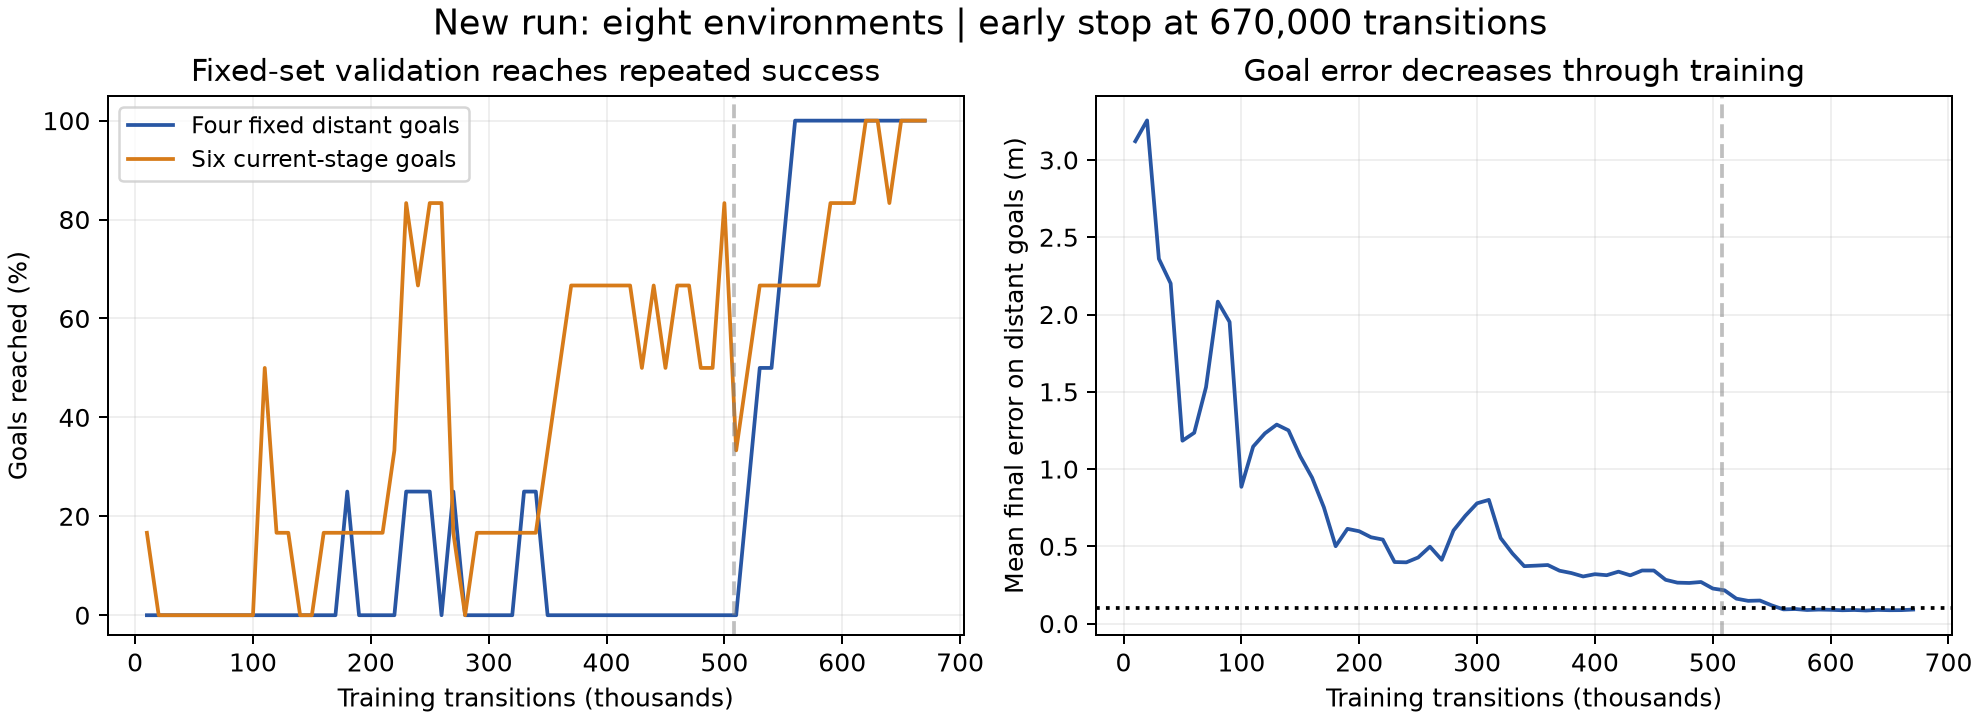
\includegraphics[width=\textwidth]{learning_progress.png}
\caption{Validation history for the reported eight-environment run. The dashed vertical line marks 507,904 transitions, the end of the earlier same-seed run. Current-stage goals change on curriculum promotion. The repeated end-of-training validation is counted only once in this plot.}\label{fig:learning}
\end{figure}

The run contains 1,639 completed training episodes: 655 goals, 917 timeouts and 67 out-of-bounds terminations. These totals include early unsuccessful learning. In the final hundred episodes, ninety succeed. After the full goal distribution is enabled, 336 of 461 completed episodes succeed and no out-of-bounds termination is recorded. These observations indicate improvement during learning, but do not independently certify the final deterministic policy.

The selected checkpoint at 630,000 transitions passes the four distant goals and all six stage goals. The final model also passes both sets. They differ because selection uses a lexicographic validation score, not simply the most recent training step. Both are retained and evaluated to make this distinction explicit.

\section{Additional goal-reaching tests}
Table~\ref{tab:goals} and Figure~\ref{fig:goals} report the sixty-goal evaluation. Both checkpoints achieve 59/60 successes, or 98.3\% observed success. This is a count on the specified evaluation set, not an estimated universal success probability. The obstacle is distant in these trials, so the measurement concerns navigation without active obstacle avoidance.

\begin{table}[htbp]\centering
\caption{Additional goal tests; twenty goals per distance group.}\label{tab:goals}
\begin{tabular}{lrrrr}\toprule
& \multicolumn{2}{c}{Validated 630k} & \multicolumn{2}{c}{Final 670k}\\
Group & Success & Mean error (m) & Success & Mean error (m)\\\midrule
Near & 20/20 & 0.0815 & 20/20 & 0.0795\\
Medium & 20/20 & 0.0812 & 20/20 & 0.0675\\
Distant & 19/20 & 0.0834 & 19/20 & 0.0851\\\bottomrule
\end{tabular}\end{table}
\begin{figure}[htbp]\centering
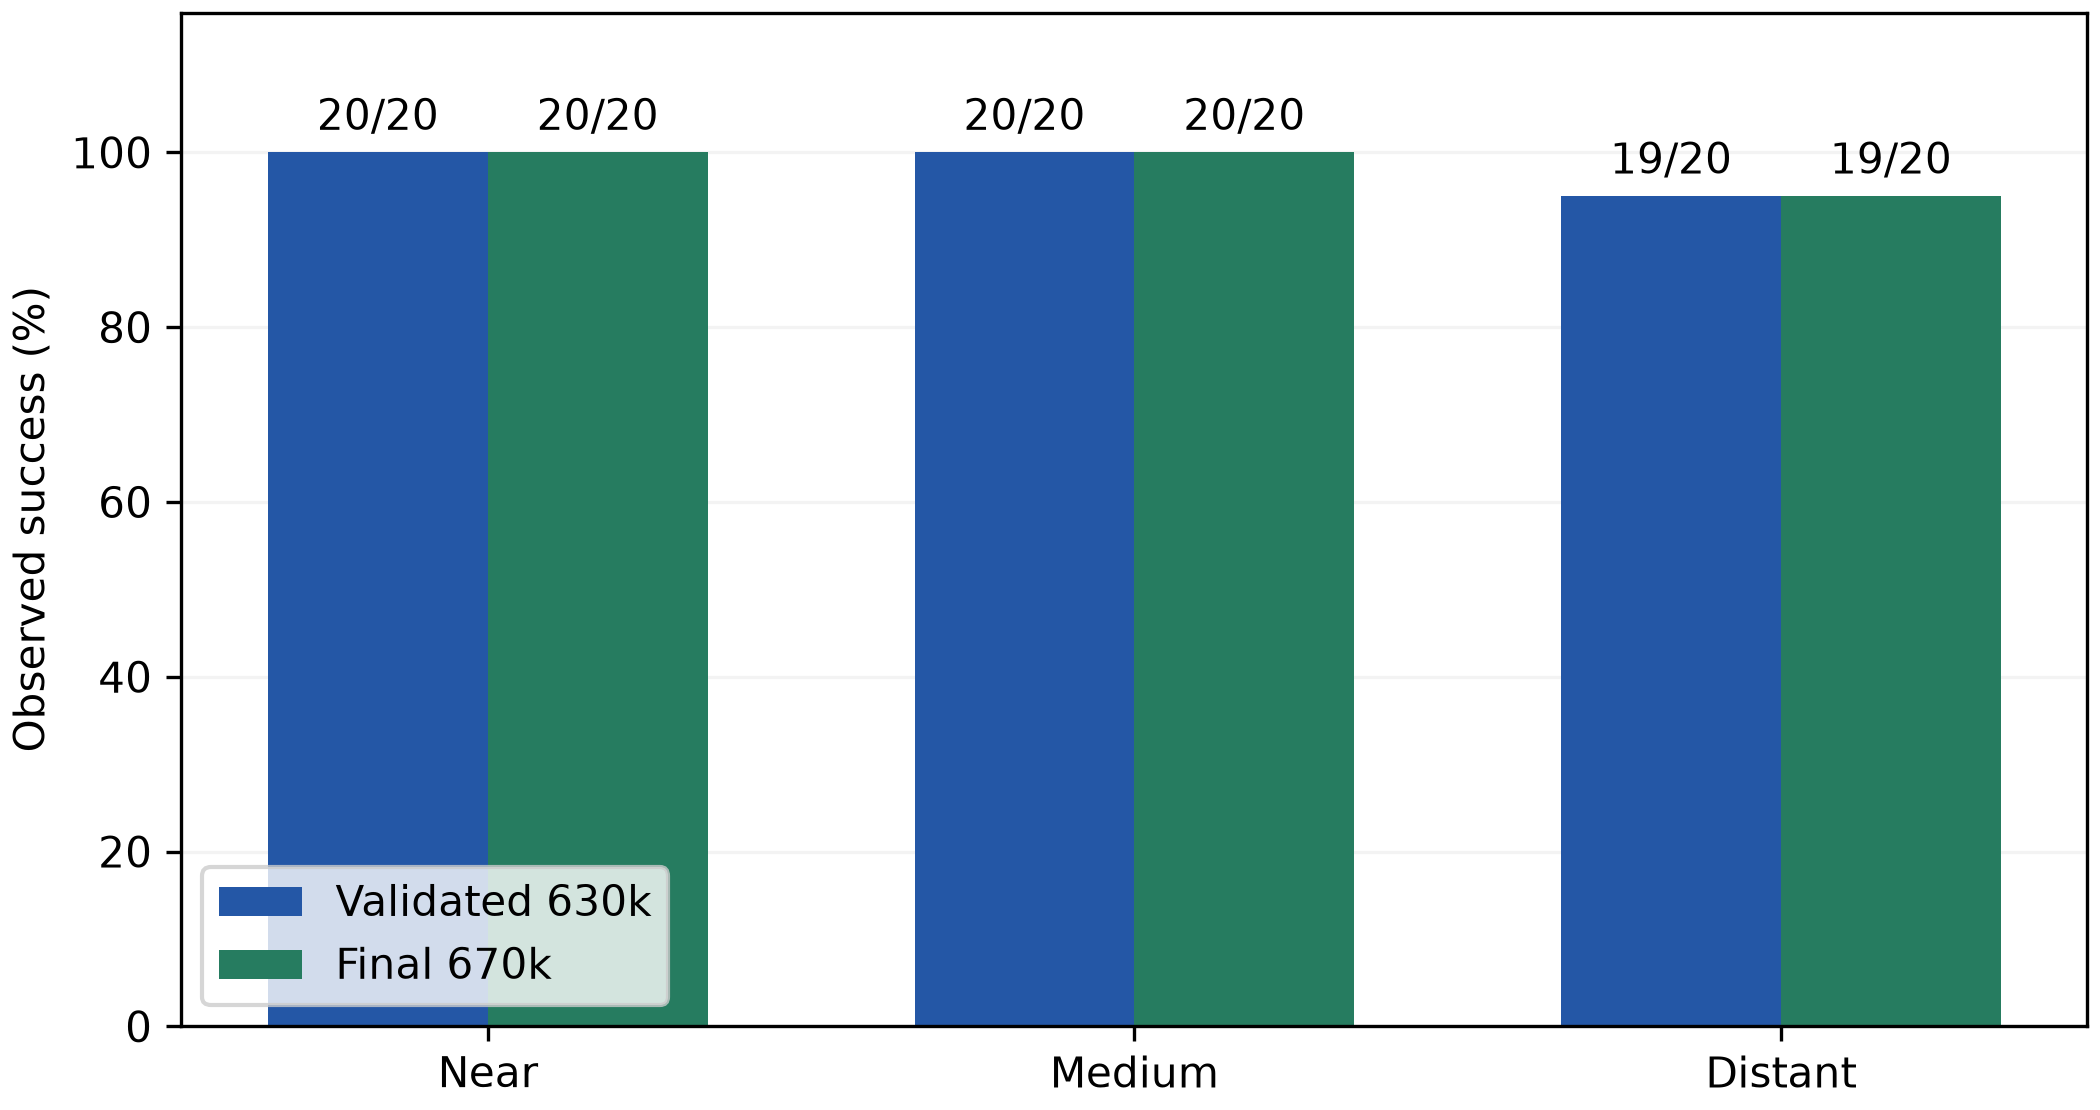
\includegraphics[width=.80\textwidth]{goal_generalization.png}
\caption{Observed success on the same additional goal set for the two checkpoints. No out-of-bounds event occurred in these tests.}\label{fig:goals}
\end{figure}

Both policies fail the same target, approximately $[0.9412,-4.7667,2.9977]^\mathsf{T}$~m. The selected checkpoint finishes 0.1097~m away and the final checkpoint 0.1344~m away. Their closest distances are 0.1021 and 0.1034~m, respectively: neither enters the original 0.10~m acceptance radius. Their final speeds are small, indicating a residual position offset rather than a high-speed pass through the target. The tolerance is not relaxed to convert this failure into a success.

The final model averages 6.42~s over the sixty episodes, including the timeout, compared with 7.20~s for the selected model. This aggregate mixes short and long tasks and should not be interpreted as the time required for the separate five-metre scenario mission. It also shows that the selected and final models are not uniformly ordered on every metric.

\section{Scenario results for the selected model}
Table~\ref{tab:selected} uses only the automatically selected 630,000-step checkpoint. All nine controller/scenario combinations reach the shared goal. The nominal PPO is identical between pure RL and RL+ACBF. Figure~\ref{fig:comparison} summarizes arrival and separation, and Figure~\ref{fig:goalerrors} shows the goal-error histories.

\begin{table}[htbp]\centering\small
\caption{Main scenario results for the validated checkpoint. $d_{\min}$ is centre separation, not surface clearance. Cases 1--3 are linear, accelerating and figure-eight motion.}\label{tab:selected}
\begin{tabular}{llrrrr}
\toprule
Case & Controller & Time (s) & Error (m) & $d_{\min}$ (m) & Path (m)\\
\midrule
1 & Pure RL & 13.70 & 0.089 & 2.067 & 7.628 \\
1 & RL+ACBF & 13.70 & 0.089 & 2.067 & 7.628 \\
1 & PID+ACBF & 7.60 & 0.086 & 1.828 & 5.087 \\
\addlinespace
2 & Pure RL & 13.70 & 0.089 & 1.072 & 7.628 \\
2 & RL+ACBF & 13.80 & 0.088 & 1.211 & 7.386 \\
2 & PID+ACBF & 7.85 & 0.087 & 1.003 & 5.095 \\
\addlinespace
3 & Pure RL & 13.70 & 0.089 & 0.464 & 7.628 \\
3 & RL+ACBF & 13.60 & 0.078 & 0.770 & 7.441 \\
3 & PID+ACBF & 7.80 & 0.085 & 0.842 & 5.099 \\
\bottomrule
\end{tabular}
\end{table}
\begin{figure}[htbp]\centering
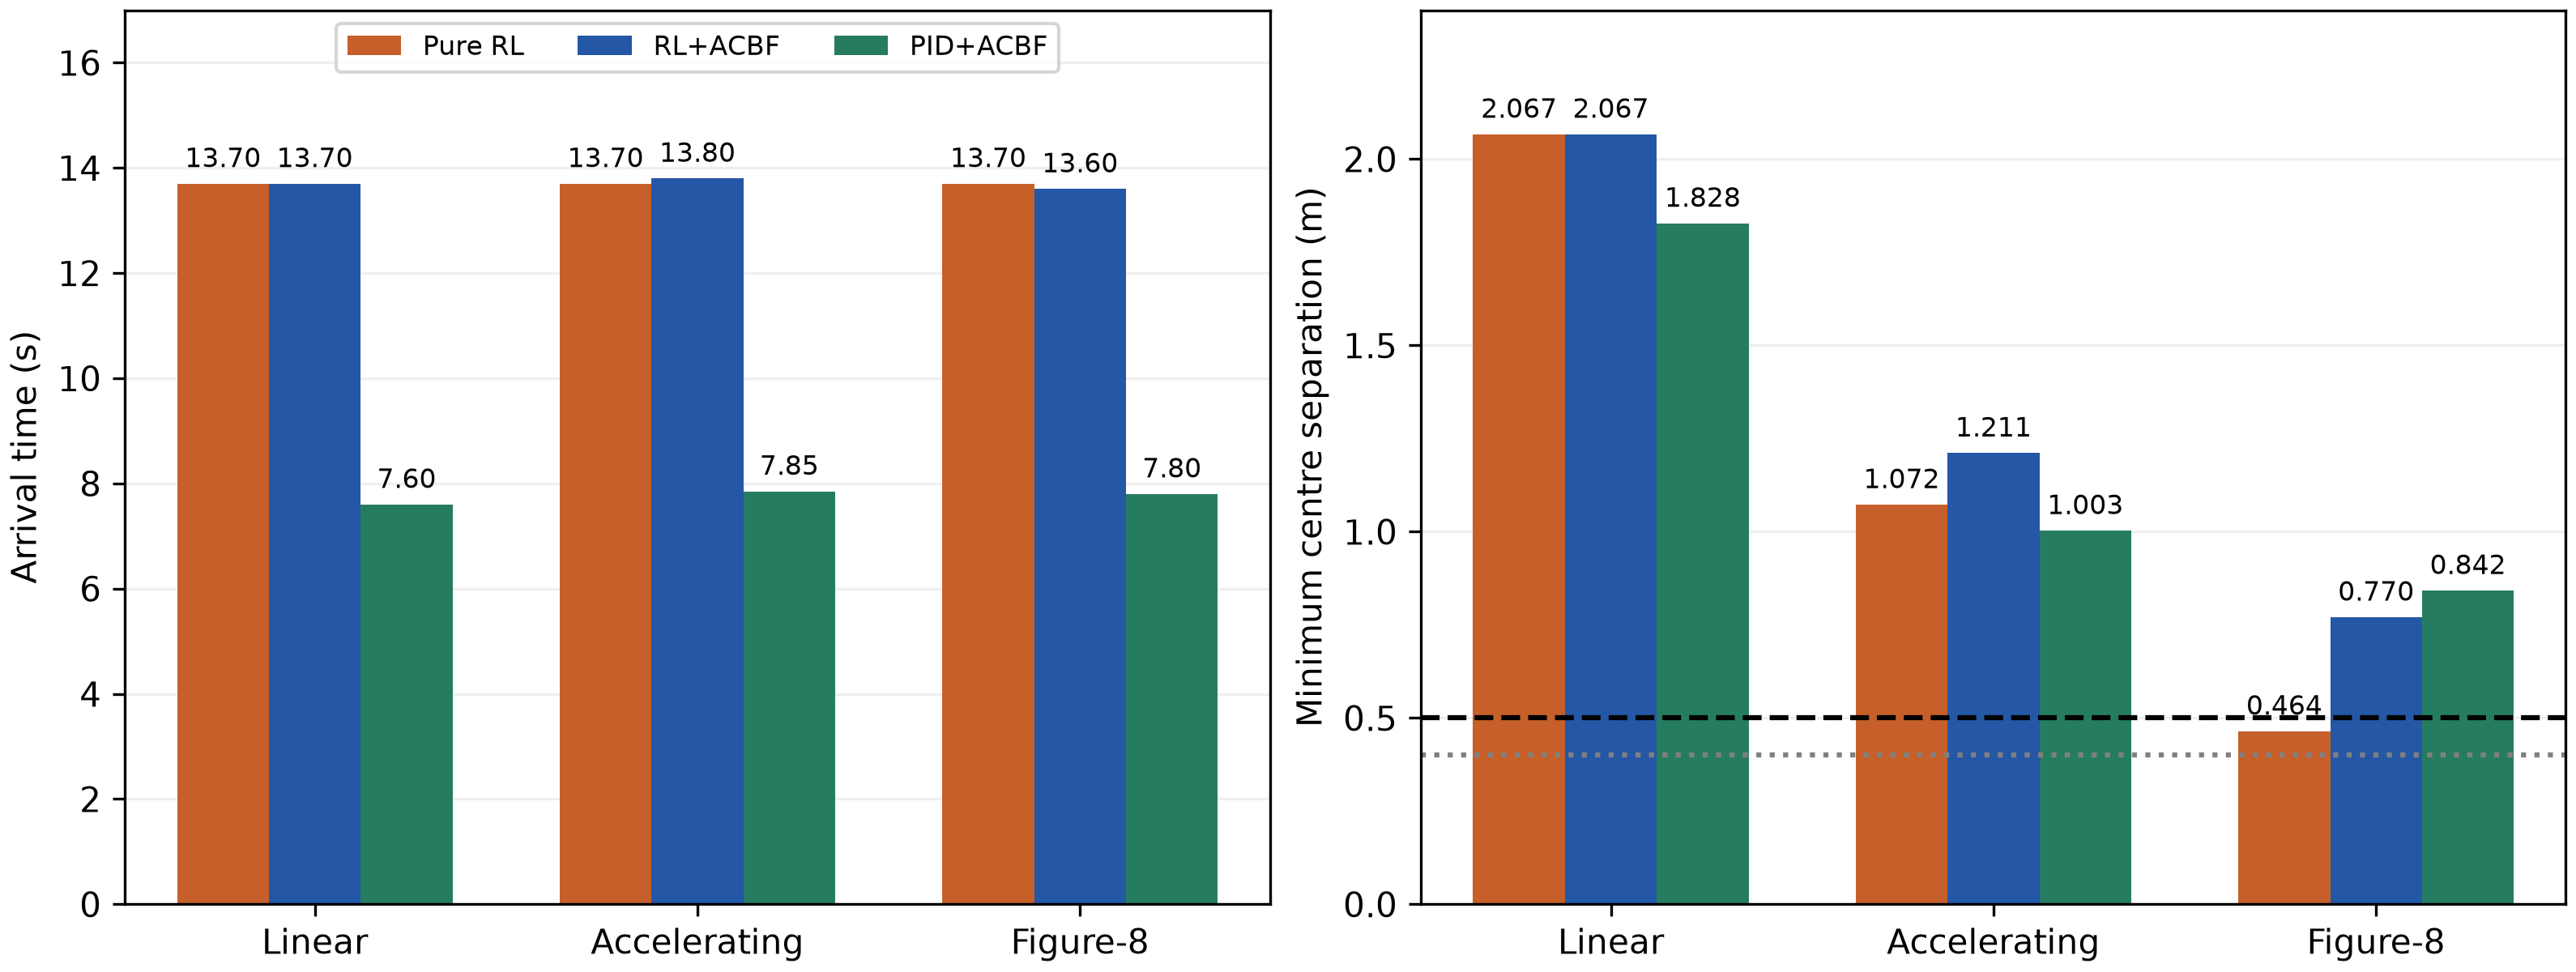
\includegraphics[width=\textwidth]{selected_comparison.png}
\caption{Selected-checkpoint comparison. In the right panel the dashed line is the 0.50~m safety boundary and the dotted line is the 0.40~m collision threshold.}\label{fig:comparison}
\end{figure}
\begin{figure}[htbp]\centering
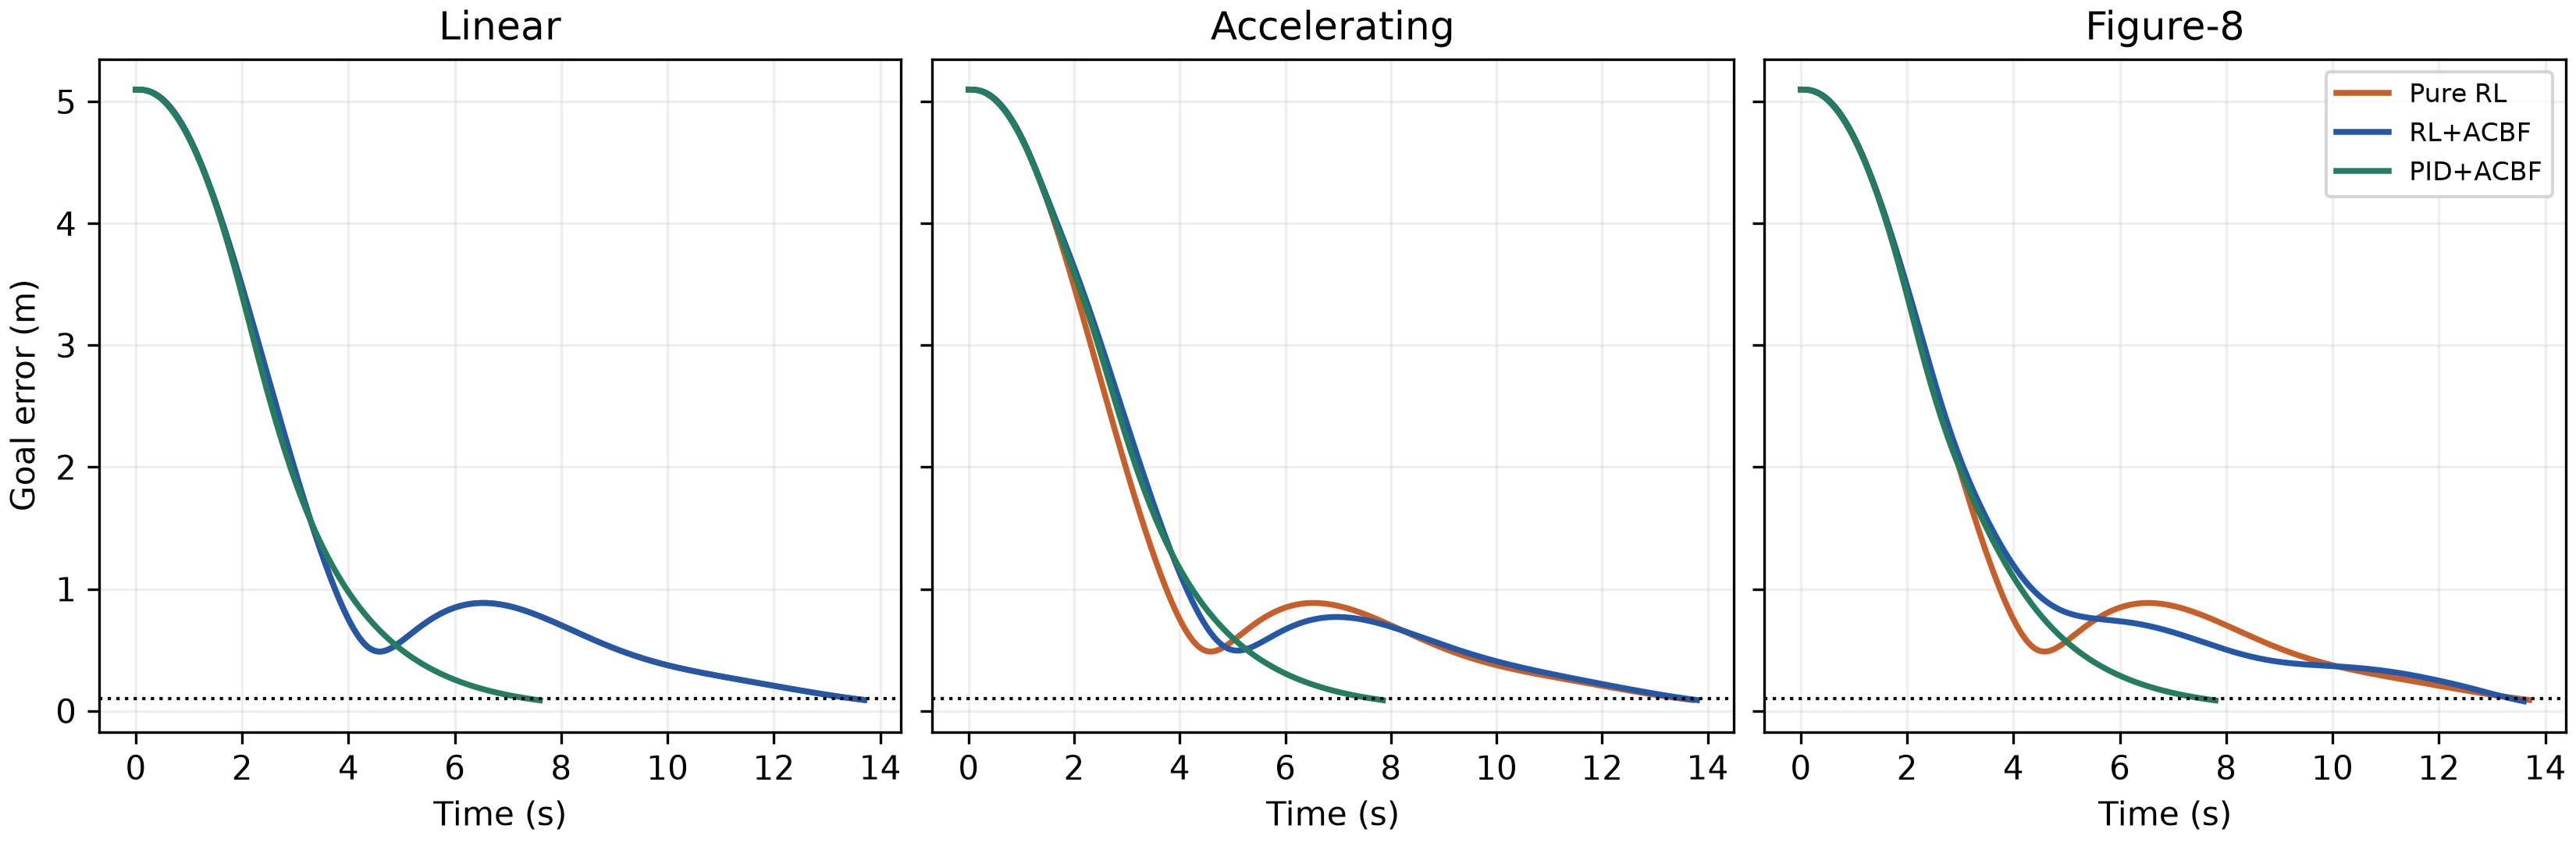
\includegraphics[width=\textwidth]{selected_goal_errors.png}
\caption{Goal-error histories for the selected checkpoint. The dotted horizontal line is the 0.10~m position tolerance; arrival additionally requires the speed and hold-time conditions.}\label{fig:goalerrors}
\end{figure}

\subsection{Linear obstacle}
In case 1, pure RL and RL+ACBF have the same trajectory and arrive in 13.70~s. Their minimum centre distance is 2.067~m, comfortably above the buffer boundary. The nominal trajectory does not require alteration by the filter in this case. PID+ACBF reaches the goal in 7.60~s with a shorter path. Thus the filter's pass-through behavior can be observed without implying an efficiency advantage for RL.

\begin{figure}[htbp]\centering
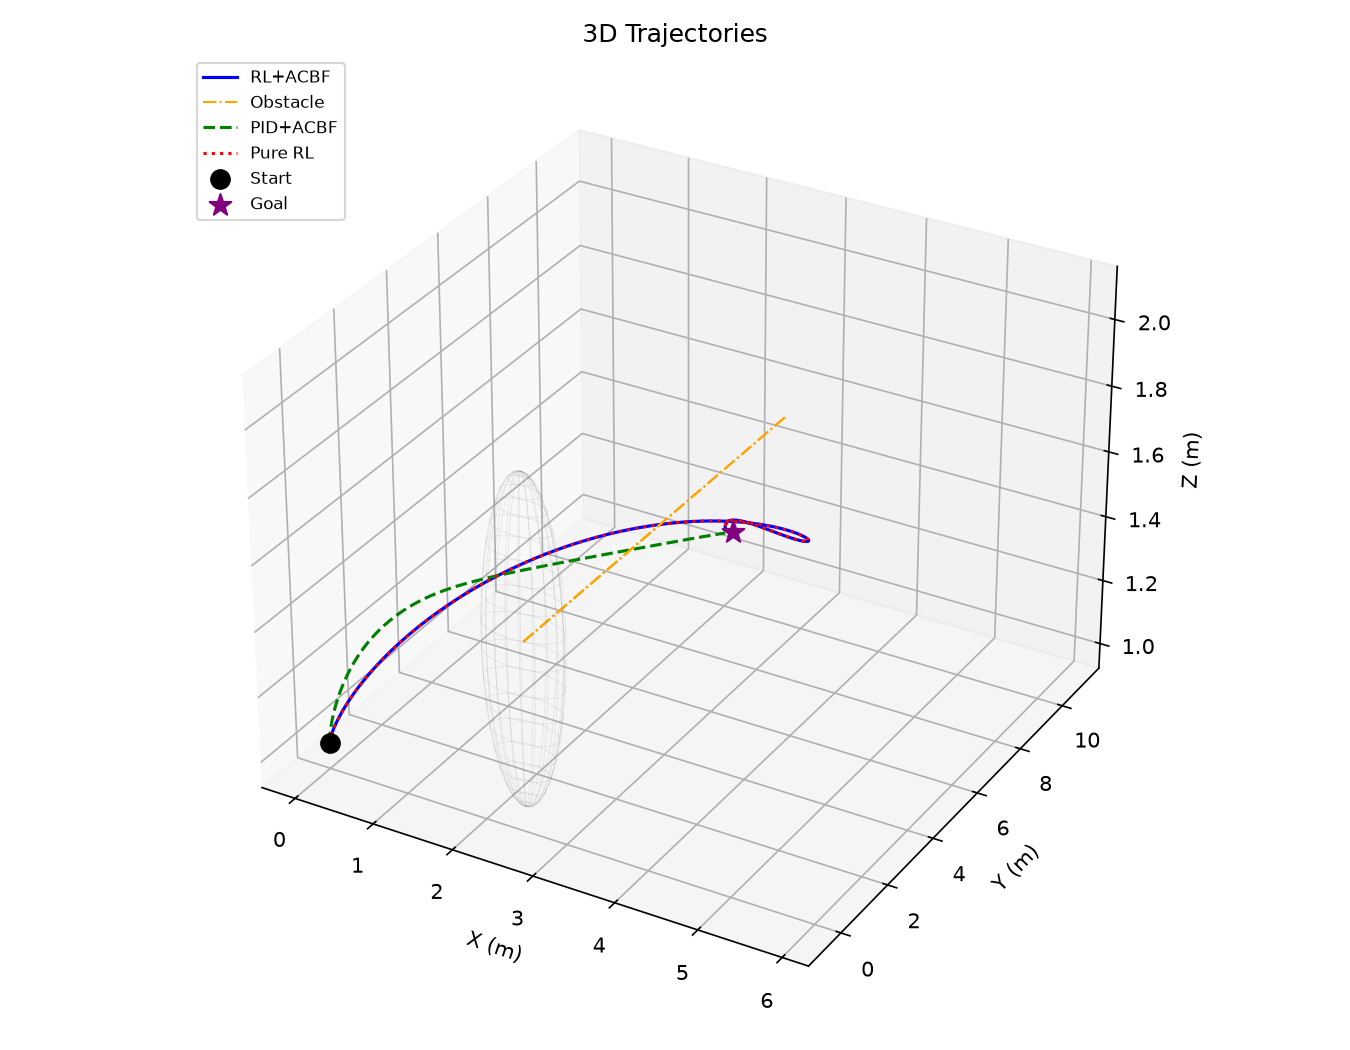
\includegraphics[width=.72\textwidth]{case1_trajectory.png}
\caption{Case 1 trajectories for the selected checkpoint. A spatial trajectory plot does not by itself establish time-aligned obstacle clearance; that is measured from the logged states.}\label{fig:case1}
\end{figure}

\subsection{Accelerating obstacle}
In case 2, the obstacle accelerates across the nominal flight region. Adding ACBF increases minimum centre separation from 1.072 to 1.211~m. Arrival changes from 13.70 to 13.80~s, while sampled path length decreases from 7.628 to 7.386~m. A filter-induced change in state can affect the later policy trajectory, so a larger safety distance does not necessarily imply a longer path. These are measured outcomes for this case, not a general optimality statement.

\begin{figure}[htbp]\centering
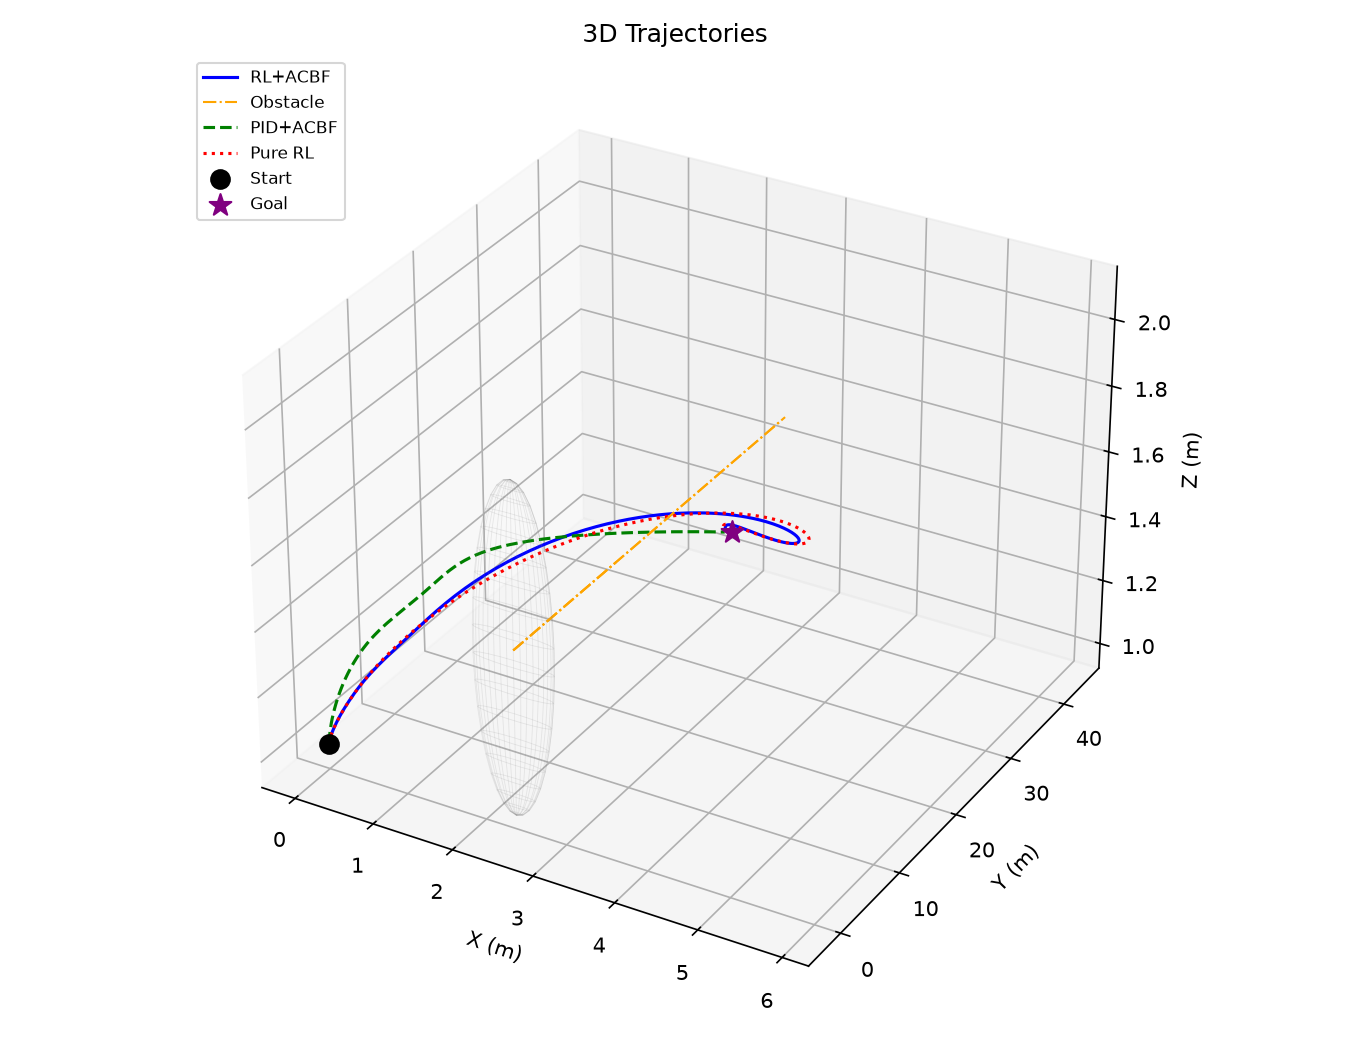
\includegraphics[width=.72\textwidth]{case2_trajectory.png}
\caption{Case 2 trajectories for the selected checkpoint. Both RL variants arrive, while the filtered path maintains a larger sampled minimum separation.}\label{fig:case2}
\end{figure}

\subsection{Figure-eight obstacle}
Case 3 is the clearest demonstration of the filter's measured safety-buffer benefit. Pure RL reaches the goal but attains a minimum centre distance of 0.464~m. This is below the 0.50~m safety boundary and above the 0.40~m geometric collision threshold. It is a buffer violation, not a recorded collision.

RL+ACBF maintains a minimum centre distance of 0.770~m and reaches the goal in 13.60~s. The increase in minimum separation is approximately 0.306~m. Surface clearance changes from 0.064 to 0.370~m. The filtered trajectory also arrives 0.10~s earlier than pure RL. This small time difference should not be interpreted as a reliable speed advantage across tasks, but it shows that preserving the observed buffer need not prevent arrival.

\begin{figure}[htbp]\centering
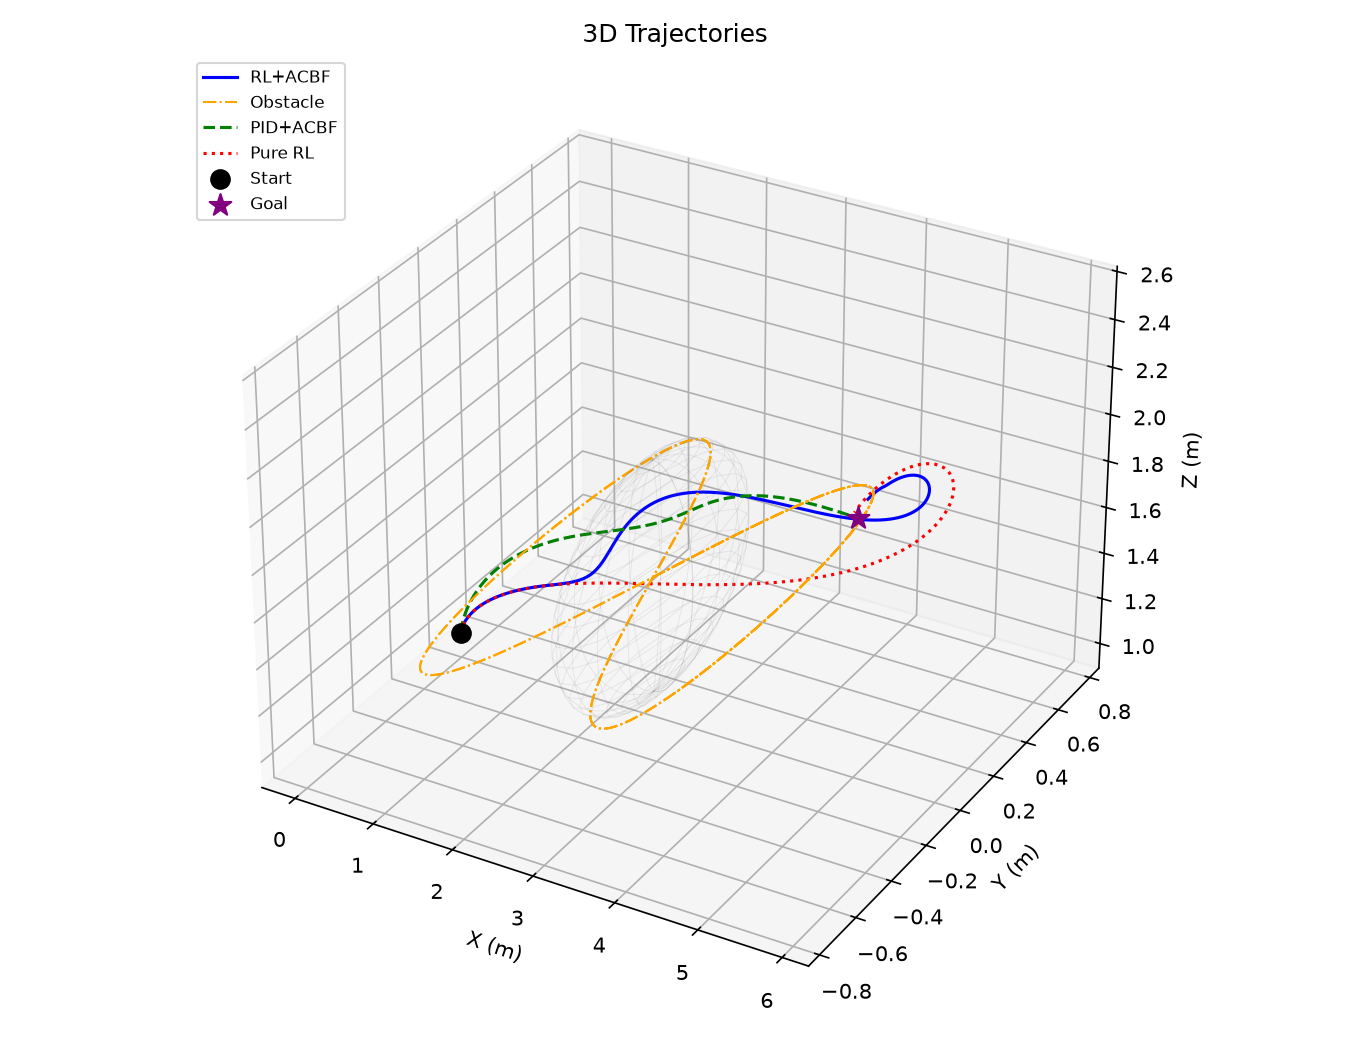
\includegraphics[width=.72\textwidth]{case3_trajectory.png}
\caption{Case 3 trajectories for the selected checkpoint. PPO+ACBF and PID+ACBF use the same obstacle predictor and filter but different nominal commands.}\label{fig:case3}
\end{figure}
\begin{figure}[htbp]\centering
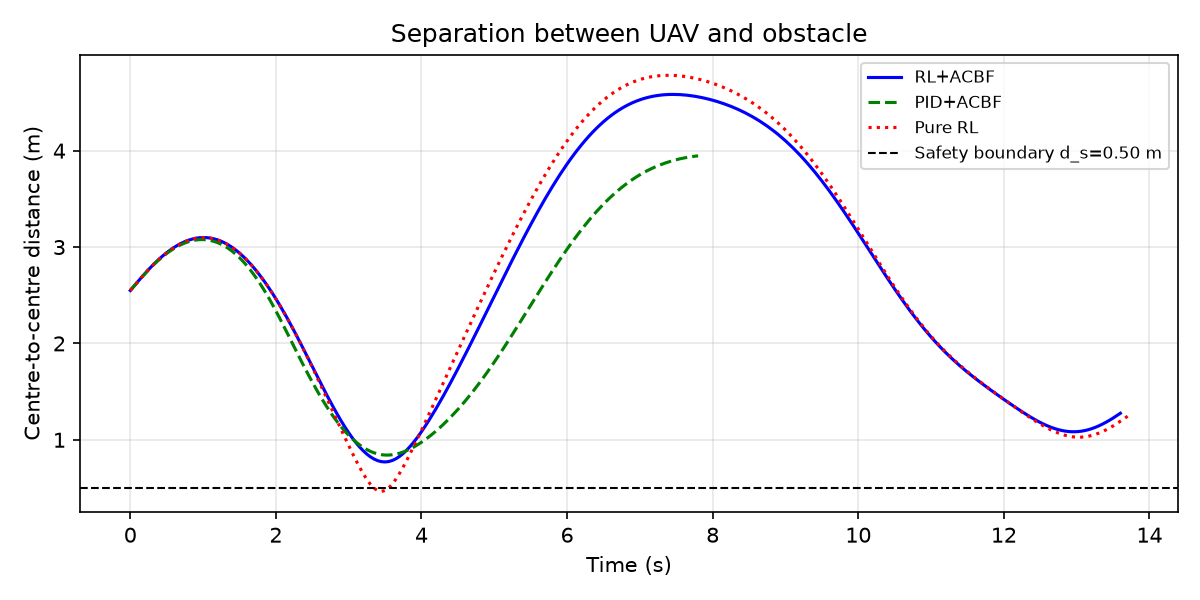
\includegraphics[width=.94\textwidth]{case3_separation.png}
\caption{Time-aligned centre separation in case 3. Pure RL enters the buffer; the filtered methods remain above it in these flights. Distance after a method's arrival is not evaluated because its episode has ended.}\label{fig:separation3}
\end{figure}

PID+ACBF reaches the goal in 7.80~s and maintains 0.842~m minimum separation. It therefore remains the stronger controller on both arrival time and minimum separation in this particular case. More generally, its mean scenario arrival time is 7.75~s, compared with 13.70~s for selected PPO+ACBF. The local results do not support a claim that RL is superior to PID on all evaluated metrics.
\FloatBarrier

\section{Final-checkpoint comparison}
Table~\ref{tab:final} reports the final 670,000-step checkpoint separately. It reaches the shared goal in every case, but its behavior differs from the selected checkpoint. Pure RL takes 17.10~s in each case and enters the figure-eight buffer. ACBF preserves the buffer and leads to earlier arrival in cases 2 and 3, at 12.15 and 12.70~s. The safety filter changes the entire subsequent closed-loop trajectory, so it can sometimes improve arrival time even though its objective is to stay close to the nominal command at each sample.

\begin{table}[htbp]\centering\small
\caption{Separate comparison using the final 670,000-step checkpoint. PID rows are repeated for consistent comparison and are not independent repeated trials.}\label{tab:final}
\begin{tabular}{llrrrr}
\toprule
Case & Controller & Time (s) & Error (m) & $d_{\min}$ (m) & Path (m)\\
\midrule
1 & Pure RL & 17.10 & 0.097 & 2.042 & 7.198 \\
1 & RL+ACBF & 17.10 & 0.097 & 2.042 & 7.198 \\
1 & PID+ACBF & 7.60 & 0.086 & 1.828 & 5.087 \\
\addlinespace
2 & Pure RL & 17.10 & 0.097 & 1.040 & 7.198 \\
2 & RL+ACBF & 12.15 & 0.096 & 1.186 & 6.799 \\
2 & PID+ACBF & 7.85 & 0.087 & 1.003 & 5.095 \\
\addlinespace
3 & Pure RL & 17.10 & 0.097 & 0.465 & 7.198 \\
3 & RL+ACBF & 12.70 & 0.085 & 0.749 & 6.853 \\
3 & PID+ACBF & 7.80 & 0.085 & 0.842 & 5.099 \\
\bottomrule
\end{tabular}
\end{table}

The final and selected models tie on additional goal success but differ in arrival times and the residual error of their shared failed goal. Retaining both provides a more complete picture than reporting whichever checkpoint is best for each metric. The results in the main trajectory figures all use the selected checkpoint.

\section{Diagnosis of earlier near-goal failures}
An earlier run's selected checkpoint at 340,000 transitions approached the scenario goal but stopped outside the tolerance. Pure RL finished approximately 0.424~m away after 25~s. Extending an obstacle-distant diagnostic flight to 60~s left it almost stationary 0.407~m away. A static policy probe found a zero-command position matching that endpoint closely. This identified a learned position bias, rather than merely insufficient episode duration.

Translated short-distance tests provided further evidence: the same 0.2~m relative movement succeeded near the fixed training start but failed near the distant scenario target. Since the observation contains absolute position, a policy can learn different local responses at different locations. The curriculum's early concentration around a fixed start is a plausible contributor. However, no controlled retraining ablation has established that removing absolute position alone would fix this behavior. The latest model substantially reduces the problem, but the remaining distant-goal timeout shows that precise positioning is not perfect everywhere.

\section{Computational and safety limitations}
For the selected PPO+ACBF checkpoint, recorded 95th-percentile control times are approximately 23.4, 116.2 and 118.8~ms in cases 1--3. The intended control interval is 50~ms. These timing measurements were collected during concurrent diagnostic work, so an isolated benchmark is required before drawing a hardware-speed conclusion. Nevertheless, the current measurements do not demonstrate real-time feasibility. Simulation arrival times must not be presented as wall-clock execution times.

The selected PPO+ACBF runs include one accepted inaccurate-solver step in case 2 and three in case 3. The implementation checks finite values and numerical residuals before accepting commands, but also permits higher-order slack. Successful geometry in these flights is an empirical result, not a proof that all barrier conditions hold exactly under every forecast error.

A previous checkpoint exposed a more serious limitation: in a figure-eight encounter, obstacle prediction overestimated next-step separation, the measured distance entered the safety buffer, and the following optimization was infeasible. The current policy avoids that failure in the tested trajectories, but no change to the predictor or filter has eliminated the underlying risk. Better navigation can reduce difficult encounters without making the safety layer universally robust.

\section{Threats to validity}
The results use a single training seed. The two reported checkpoints come from one run and must not be counted as independent learning repetitions. The additional goals are reused evaluation goals. The moving-obstacle cases share a start and destination, so three successful cases do not constitute three distinct destination-generalization tests. The environment uses prescribed obstacle motion and exact simulated position measurements, not a hardware perception stack.

There is no fixed-CBF baseline, no predictor ablation and no multiple-obstacle test. Therefore the study can attribute the paired difference to adding the complete IMM/ACBF layer for the same PPO policy, but cannot isolate how much of that difference comes from adaptation, the predictor, or other implementation choices. Collision counts are geometric, sampled metrics, and zero observed collisions in a finite set is not a universal probability statement.

\section{Discussion}
The evidence supports three conclusions. First, the implemented training procedure produces substantially improved navigation and satisfies its configured stopping condition. Second, the lower layer prevents the observed figure-eight buffer entry while retaining goal arrival for the evaluated policies. Third, the classical baseline remains faster and more direct. Together these results demonstrate a working hierarchical comparison with useful diagnostics, while defining clear boundaries on what can be claimed.

The most productive next step is broader validation rather than automatically increasing the training budget to its original ceiling. Independent seeds, varied start positions, new goal sets, prediction-error tests and isolated timing measurements would address the most consequential remaining uncertainties.

\chapter{Conclusions and Future Work}\label{ch:conclusion}
\section{Conclusions}
This project implemented a hierarchical UAV navigation controller that combines PPO reference commands, IMM obstacle prediction and an adaptive barrier-based safety filter. The implementation was evaluated against pure PPO and a classical PID-based controller using the same simulated plant and arrival conditions. Configuration snapshots, checkpoint hashes and per-step logs were used to make the comparisons traceable.

The latest run stopped at 670,000 transitions after repeatedly passing its fixed validation criteria. The selected checkpoint at 630,000 transitions and the final checkpoint each reached 59 of 60 additional goals. One distant target retained a small steady position error beyond the 0.10~m radius. Thus the configured validation objective was achieved, but arbitrary-goal reliability was not established.

All three controllers reached the common destination in the linear, accelerating and figure-eight obstacle scenarios. For the selected checkpoint, the figure-eight pure-RL path entered the safety buffer with a minimum centre separation of 0.464~m. PPO+ACBF maintained 0.770~m and reached the goal in 13.60~s. This is a concrete observed benefit of the complete filtering layer. It is not a claim that a physical collision was prevented, because the unfiltered trajectory did not cross the configured collision threshold.

The PID-based baseline remained more efficient, reaching the scenario goal in approximately 7.6--7.85~s. The contribution is therefore a successful implementation, comparison and diagnosis of a hierarchical learning-and-filtering approach, rather than demonstrated superiority over classical control. Earlier failures and current timing limitations show why numerical prediction-based safety must be assessed beyond a favorable trajectory plot.

\section{Future work}
\textbf{Navigation generalization.} Repeat training with independent seeds and evaluate on new goals and starting states. Maintain close-to-goal tasks at varied locations after curriculum promotion to test and reduce location-dependent position bias. Use separate model-selection and final-evaluation sets.

\textbf{Prediction robustness and feasibility.} Introduce controlled sensor noise, obstacle acceleration changes and model mismatch. Evaluate margins that account for prediction uncertainty. Develop and test a feasible backup control strategy, since terminating an evaluation on solver failure is not an emergency behavior for a real drone.

\textbf{Component ablations.} Compare adaptive and fixed barrier coefficients, single-model and IMM predictions, and alternative nominal controllers under the same conditions. This would distinguish the contribution of individual components from the effect of the complete hierarchy.

\textbf{Computational validation.} Measure timing in isolated runs and profile the repeated simulator forecasts and optimization. Demonstrate deadline compliance before considering hardware deployment. Hardware-in-the-loop and physical tests should follow only after the simulation assumptions and recovery behavior are made explicit.

\textbf{Broader scenarios.} Extend the setting to multiple obstacles, varying goal locations and disturbances. Report both mission completion and safety events, retaining failures rather than relaxing criteria after observing results. These steps would turn the current successful demonstrations into stronger evidence of repeatable navigation performance.

\printbibliography[heading=bibintoc,title={References}]
\appendix
\chapter{Reproducibility and Artifacts}\label{app:repro}
\section{Experiment identity}
The main results come from local project artifacts \parencite{projectdata}. Training run: \texttt{20261105T022305\_489044Z}. Evaluation root: \texttt{20261105T081629\_168420Z}. The experiment source fingerprint, using ordered relative Python paths and LF-normalized file bytes, is
\begin{quote}\small\ttfamily
e27217395c51bdde1b11697346c61b5e5\allowbreak ea5a16e159b46739ebe0317d3d758f1.
\end{quote}
The selected \texttt{best\_candidate.zip} and \texttt{validated\_model.zip} are identical. Their SHA-256 is
\begin{quote}\small\ttfamily
0b58672c4e2d794b19e04e02ef9c4c56\allowbreak ab091c087481f23aa9d7b45f1d23bd1a.
\end{quote}
The final model SHA-256 is
\begin{quote}\small\ttfamily
ae7a2a0049fb52dbafc69a7d99184964\allowbreak 42694bd0fd4d1cce843fd426c12a590c.
\end{quote}
Hashes were verified unchanged after inference. The selected model has 630,000 recorded transitions and the final model 670,000. Both are in the full-distribution curriculum stage.

\section{Recorded dependencies}
\begin{table}[htbp]\centering
\caption{Versions recorded in the training manifest.}\label{tab:versions}
\begin{tabular}{ll}\toprule Component & Version\\\midrule
Python & 3.14.3\\NumPy / SciPy & 2.5.3 / 1.18.0\\
PyTorch & 2.14.1+cu126\\Gymnasium & 1.3.0\\
Stable-Baselines3 & 2.9.0\\PyBullet & 3.2.7\\
gym-pybullet-drones & 2.2.0\\CVXPY & 1.9.3\\
CLARABEL / SCS & 0.11.1 / 3.3.1\\
Matplotlib & 3.11.2\\\bottomrule
\end{tabular}\end{table}
These are recorded environment versions, not a claim that every later library version reproduces identical trajectories. The report does not infer hardware speed from these package versions.

\section{Evaluation commands}
The following command evaluates the selected checkpoint and creates a new dated output directory. It does not train a policy.
\begin{lstlisting}[language={},caption={Evaluate the selected policy on all three scenarios.}]
python evaluate.py --model results/training/20261105T022305_489044Z/validated_model.zip --case all
\end{lstlisting}
For the final-policy comparison, replace the filename by \texttt{ppo\_final.zip}. The saved evaluation runner in the review directory performs the sixty-goal tests and blocks learning calls. It uses the stored coordinates and seeds to keep the checkpoint comparison paired. A rerun should use a new output directory rather than overwrite prior evidence.

\section{Figure inventory}
The main external figure files are listed below. Every trajectory and separation figure uses the selected 630,000-step checkpoint. The training figure covers the whole run; the additional-goal figure explicitly compares both checkpoints. A machine-readable \texttt{figure\_sources.json} is included in the Overleaf package.

\begin{longtable}{p{.44\textwidth}p{.49\textwidth}}
\caption{Figure files and their role.}\label{tab:figures}\\
\toprule File in \texttt{figures/} & Purpose\\\midrule\endfirsthead
\toprule File & Purpose\\\midrule\endhead
\texttt{learning\_progress.png} & Fixed and stage validation history\\
\texttt{goal\_generalization.png} & Additional goal success for 630k and 670k\\
\texttt{selected\_comparison.png} & Main arrival and separation comparison\\
\texttt{selected\_goal\_errors.png} & Goal-error curves for the selected policy\\
\texttt{case1\_trajectory.png} & Linear-obstacle 3D trajectories\\
\texttt{case2\_trajectory.png} & Accelerating-obstacle 3D trajectories\\
\texttt{case3\_trajectory.png} & Figure-eight 3D trajectories\\
\texttt{case3\_separation.png} & Figure-eight time-aligned safety evidence\\
\texttt{case1\_separation.png} & Supplementary linear-case distance history\\
\texttt{case2\_separation.png} & Supplementary accelerating-case distance history\\\bottomrule
\end{longtable}

\begin{figure}[htbp]\centering
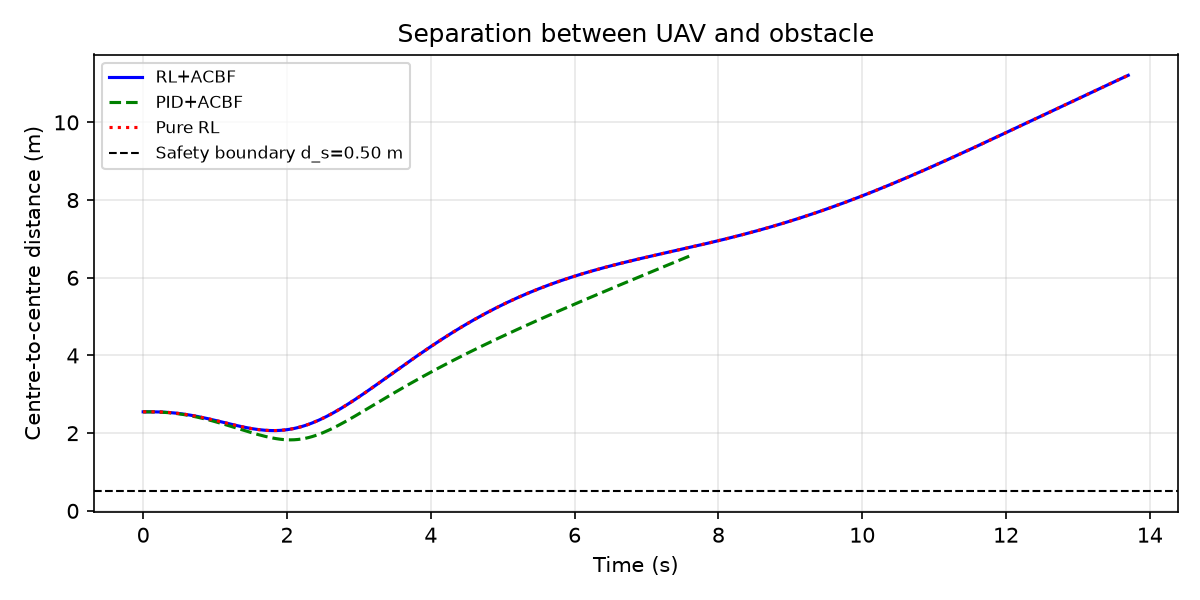
\includegraphics[width=.92\textwidth]{case1_separation.png}
\caption{Supplementary case 1 separation history for the selected checkpoint.}\label{fig:separation1}
\end{figure}
\begin{figure}[htbp]\centering
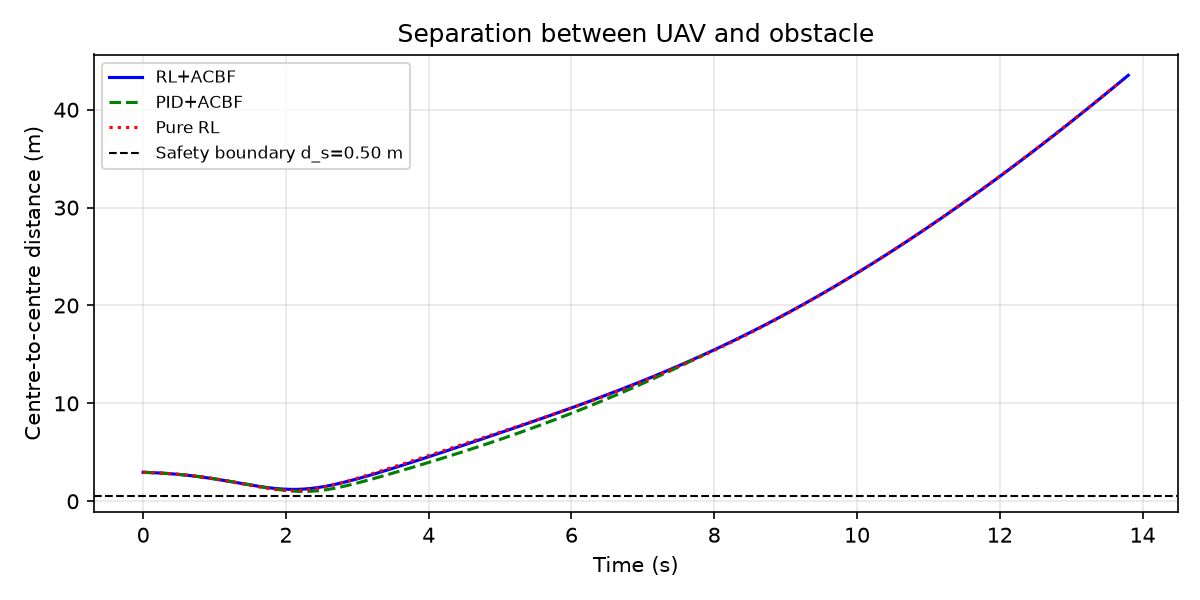
\includegraphics[width=.92\textwidth]{case2_separation.png}
\caption{Supplementary case 2 separation history for the selected checkpoint.}\label{fig:separation2}
\end{figure}

\section{Interpretation checklist}
An arrival claim must use both position and speed/hold conditions. A safety claim must distinguish the 0.50~m buffer from the 0.40~m collision threshold. A checkpoint comparison must identify the actual weights used. A generalization claim must identify which goals and training seeds were tested. A real-time claim requires wall-clock deadline measurements. These distinctions are necessary to reproduce the conclusions of this report without overstating the evidence.

\end{document}
